% 图 64.4 —— 由 `checks/emit_hand.py` 自动拼出（probe 精测 + prims2 图元分解）
%%
% ⚠ 这是**稿子不是成品**：跑 `checks/checkhand.py 64.4` 看指标 + 看叠合图。
%%
%% ⚠ 待核：
%   · 本图 probe 报出阴影族 3 个 —— **本脚本不生成阴影**（要照原书手写）；prims2 的 strokes 里可能含阴影线，核对时留意别画重
%   · 可疑字形 1 项（空心圈 ⊙ 常被认成字母 o）—— 见文件末
%%
\documentclass[12pt]{standalone}
\usepackage{fontspec}
\setsansfont{Arial}
\newfontfamily\mfallback{DejaVu Sans}
\usepackage{tikz}
\begin{document}
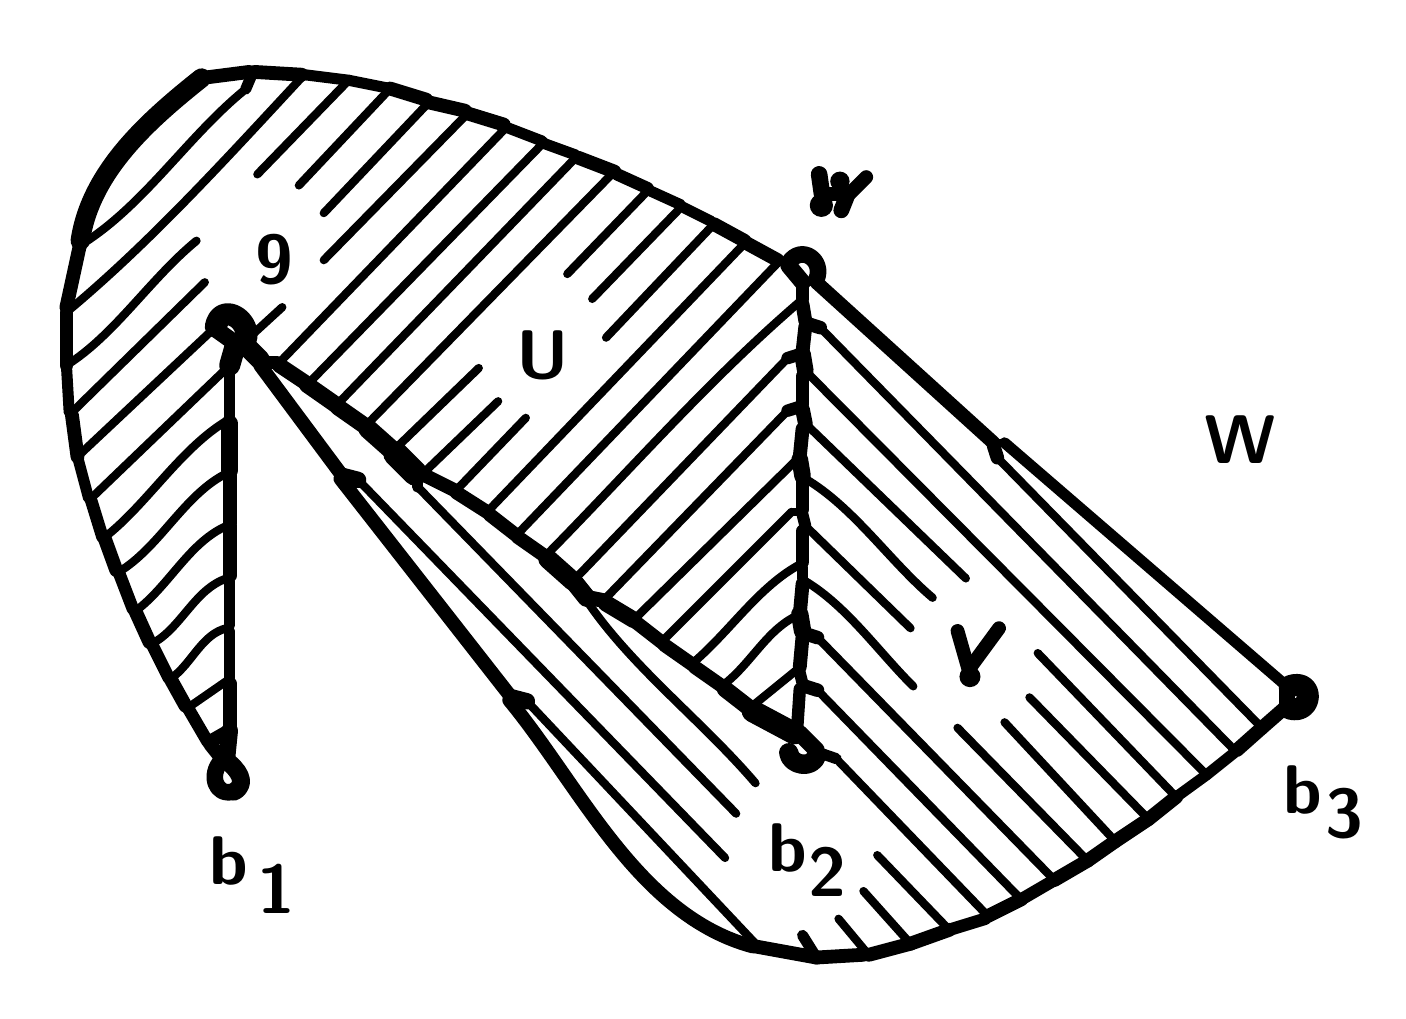
\begin{tikzpicture}[x=1pt, y=-1pt, line width=3.0pt, line cap=round, line join=round]

  %% ════ 填充区（prims2 的 fills）════

  %% ════ 直线段（prims2 的 strokes）════
  \draw[line width=3.0pt] (155.0,167.0) -- (180.0,141.0);
  \draw[line width=4.0pt] (186.0,41.0) -- (173.0,36.0);
  \draw[line width=5.0pt] (349.0,150.0) -- (285.0,92.0);
  \draw[line width=3.0pt] (436.0,261.0) -- (286.4,108.4);
  \draw[line width=4.9pt] (286.4,108.4) -- (282.0,107.0);
  \draw[line width=7.0pt] (197.0,200.0) -- (188.0,192.0);
  \draw[line width=4.5pt] (33.0,197.0) -- (38.0,210.0);
  \draw[line width=5.0pt] (293.0,60.0) -- (288.0,60.0);
  \draw[line width=5.0pt] (44.0,222.0) -- (39.0,211.0);
  \draw[line width=4.0pt] (237.0,65.0) -- (247.0,70.0);
  \draw[line width=3.0pt] (383.0,301.0) -- (336.0,253.0);
  \draw[line width=5.0pt] (383.0,301.0) -- (393.0,294.0);
  \draw[line width=5.0pt] (383.0,301.0) -- (371.0,308.0);
  \draw[line width=3.0pt] (107.0,84.0) -- (158.0,32.0);
  \draw[line width=5.3pt] (203.0,206.0) -- (208.0,207.0);
  \draw[line width=4.5pt] (45.0,223.0) -- (51.0,235.0);
  \draw[line width=3.0pt] (170.0,135.0) -- (144.0,160.0);
  \draw[line width=4.0pt] (131.0,22.0) -- (116.0,19.0);
  \draw[line width=5.0pt] (131.0,22.0) -- (144.0,26.0);
  \draw[line width=3.0pt] (131.0,22.0) -- (98.0,57.0);
  \draw[line width=5.0pt] (187.0,191.0) -- (177.0,184.0);
  \draw[line width=5.0pt] (279.0,155.0) -- (280.0,145.0);
  \draw[line width=5.0pt] (73.0,198.0) -- (73.0,180.0);
  \draw[line width=3.0pt] (346.0,320.0) -- (292.1,264.1);
  \draw[line width=4.0pt] (292.1,264.1) -- (286.0,262.0);
  \draw[line width=3.0pt] (220.0,213.0) -- (278.0,156.0);
  \draw[line width=7.6pt] (75.0,115.0) -- (73.0,122.0);
  \draw[line width=3.0pt] (133.0,152.0) -- (163.0,123.0);
  \draw[line width=5.0pt] (297.0,60.0) -- (303.0,54.0);
  \draw[line width=4.9pt] (281.0,219.0) -- (285.4,220.4);
  \draw[line width=3.0pt] (285.4,220.4) -- (371.0,308.0);
  \draw[line width=4.0pt] (116.0,19.0) -- (100.0,17.0);
  \draw[line width=3.0pt] (116.0,19.0) -- (83.0,53.0);
  \draw[line width=5.0pt] (347.0,321.0) -- (359.0,315.0);
  \draw[line width=6.0pt] (73.0,160.0) -- (73.0,143.0);
  \draw[line width=3.0pt] (339.0,199.0) -- (282.0,144.0);
  \draw[line width=6.0pt] (455.0,245.0) -- (455.0,239.0);
  \draw[line width=5.0pt] (14.0,101.0) -- (19.0,78.0);
  \draw[line width=5.0pt] (174.0,241.0) -- (113.0,163.0);
  \draw[line width=5.0pt] (32.0,196.0) -- (28.0,185.0);
  \draw[line width=3.0pt] (209.0,112.0) -- (247.0,72.0);
  \draw[line width=5.0pt] (154.0,167.0) -- (144.0,162.0);
  \draw[line width=5.0pt] (18.0,155.0) -- (16.0,140.0);
  \draw[line width=3.0pt] (18.0,155.0) -- (67.0,109.0);
  \draw[line width=4.0pt] (18.0,155.0) -- (22.0,170.0);
  \draw[line width=5.9pt] (175.0,242.0) -- (180.4,243.4);
  \draw[line width=3.0pt] (180.4,243.4) -- (263.0,331.0);
  \draw[line width=3.0pt] (293.0,322.0) -- (303.0,334.0);
  \draw[line width=3.0pt] (185.0,43.0) -- (102.0,128.0);
  \draw[line width=4.9pt] (281.0,238.0) -- (285.4,239.4);
  \draw[line width=3.0pt] (285.4,239.4) -- (359.0,315.0);
  \draw[line width=5.3pt] (281.0,143.0) -- (280.0,138.0);
  \draw[line width=5.0pt] (73.0,179.0) -- (73.0,162.0);
  \draw[line width=7.1pt] (79.0,115.0) -- (84.0,120.0);
  \draw[line width=4.0pt] (73.0,218.0) -- (73.0,235.0);
  \draw[line width=4.0pt] (285.0,336.0) -- (280.0,328.0);
  \draw[line width=5.0pt] (285.0,336.0) -- (263.0,332.0);
  \draw[line width=5.0pt] (285.0,336.0) -- (302.0,335.0);
  \draw[line width=6.0pt] (112.0,137.0) -- (122.0,144.0);
  \draw[line width=6.6pt] (202.0,206.0) -- (198.0,201.0);
  \draw[line width=5.0pt] (340.0,232.0) -- (336.0,218.0);
  \draw[line width=5.0pt] (340.0,232.0) -- (351.0,217.0);
  \draw[line width=4.5pt] (224.0,58.0) -- (213.0,53.0);
  \draw[line width=3.0pt] (72.0,236.0) -- (59.0,245.0);
  \draw[line width=3.0pt] (64.0,92.0) -- (16.0,139.0);
  \draw[line width=5.0pt] (73.0,237.0) -- (73.0,254.0);
  \draw[line width=4.5pt] (371.0,308.0) -- (359.0,315.0);
  \draw[line width=6.0pt] (281.0,124.0) -- (280.0,118.0);
  \draw[line width=5.5pt] (91.0,122.0) -- (100.0,128.0);
  \draw[line width=5.7pt] (294.0,66.0) -- (296.0,61.0);
  \draw[line width=3.0pt] (259.0,78.0) -- (167.0,174.0);
  \draw[line width=6.0pt] (261.0,246.0) -- (252.0,239.0);
  \draw[line width=6.0pt] (111.0,136.0) -- (101.0,129.0);
  \draw[line width=3.0pt] (319.0,217.0) -- (282.0,181.0);
  \draw[line width=4.0pt] (73.0,141.0) -- (73.0,124.0);
  \draw[line width=3.0pt] (256.0,284.0) -- (141.0,166.0);
  \draw[line width=4.0pt] (141.0,166.0) -- (141.0,162.0);
  \draw[line width=3.0pt] (353.0,251.0) -- (393.0,294.0);
  \draw[line width=6.0pt] (280.0,162.0) -- (279.0,156.0);
  \draw[line width=5.0pt] (90.0,121.0) -- (85.0,121.0);
  \draw[line width=3.0pt] (223.0,60.0) -- (195.0,89.0);
  \draw[line width=3.0pt] (211.0,53.0) -- (123.0,143.0);
  \draw[line width=3.0pt] (177.0,183.0) -- (271.0,85.0);
  \draw[line width=3.0pt] (333.0,326.0) -- (307.0,299.0);
  \draw[line width=4.5pt] (333.0,326.0) -- (346.0,322.0);
  \draw[line width=5.0pt] (333.0,326.0) -- (319.0,331.0);
  \draw[line width=5.0pt] (281.0,108.0) -- (280.0,117.0);
  \draw[line width=4.0pt] (78.8,22.2) -- (81.0,17.0);
  \draw[line width=3.0pt] (204.0,98.0) -- (235.0,66.0);
  \draw[line width=5.0pt] (62.8,18.2) -- (80.0,16.0);
  \draw[line width=4.0pt] (187.0,42.0) -- (198.0,46.0);
  \draw[line width=5.0pt] (52.0,236.0) -- (57.0,245.0);
  \draw[line width=5.0pt] (159.0,31.0) -- (172.0,35.0);
  \draw[line width=5.0pt] (155.0,168.0) -- (166.0,175.0);
  \draw[line width=3.0pt] (92.0,101.0) -- (80.0,112.0);
  \draw[line width=4.9pt] (349.0,151.0) -- (350.4,155.4);
  \draw[line width=3.0pt] (350.4,155.4) -- (446.0,253.0);
  \draw[line width=5.0pt] (229.0,222.0) -- (220.0,215.0);
  \draw[line width=3.0pt] (144.0,28.0) -- (107.0,67.0);
  \draw[line width=5.0pt] (176.0,183.0) -- (167.0,176.0);
  \draw[line width=5.0pt] (230.0,223.0) -- (240.0,230.0);
  \draw[line width=5.0pt] (393.0,294.0) -- (405.0,286.0);
  \draw[line width=5.0pt] (251.0,238.0) -- (241.0,231.0);
  \draw[line width=4.0pt] (280.0,195.0) -- (280.0,199.0);
  \draw[line width=4.5pt] (279.0,118.0) -- (274.6,119.4);
  \draw[line width=3.0pt] (274.6,119.4) -- (198.0,199.0);
  \draw[line width=5.0pt] (304.0,335.0) -- (319.0,331.0);
  \draw[line width=6.0pt] (209.0,208.0) -- (219.0,214.0);
  \draw[line width=3.0pt] (279.0,175.0) -- (276.0,175.0);
  \draw[line width=3.0pt] (276.0,175.0) -- (230.0,221.0);
  \draw[line width=4.0pt] (436.0,262.0) -- (426.0,270.0);
  \draw[line width=5.0pt] (66.0,258.0) -- (73.0,254.0);
  \draw[line width=3.0pt] (281.0,92.0) -- (284.0,92.0);
  \draw[line width=4.3pt] (280.0,176.0) -- (281.0,180.0);
  \draw[line width=4.5pt] (279.0,137.0) -- (274.6,138.4);
  \draw[line width=3.0pt] (274.6,138.4) -- (209.0,206.0);
  \draw[line width=3.0pt] (278.0,232.0) -- (262.0,245.0);
  \draw[line width=4.0pt] (225.0,59.0) -- (236.0,64.0);
  \draw[line width=4.3pt] (279.0,233.0) -- (280.0,237.0);
  \draw[line width=6.0pt] (73.0,254.0) -- (72.0,264.0);
  \draw[line width=3.0pt] (426.0,270.0) -- (282.0,125.0);
  \draw[line width=4.0pt] (426.0,270.0) -- (415.0,278.0);
  \draw[line width=5.0pt] (212.0,52.0) -- (199.0,47.0);
  \draw[line width=6.0pt] (68.0,109.0) -- (75.0,114.0);
  \draw[line width=6.0pt] (287.0,60.0) -- (286.0,53.0);
  \draw[line width=3.0pt] (365.0,226.0) -- (415.0,278.0);
  \draw[line width=5.0pt] (281.0,106.0) -- (280.0,100.0);
  \draw[line width=5.0pt] (82.0,16.0) -- (99.0,17.0);
  \draw[line width=8.0pt] (262.0,247.0) -- (277.0,255.0);
  \draw[line width=5.0pt] (259.0,77.0) -- (248.0,71.0);
  \draw[line width=3.0pt] (23.0,170.0) -- (72.0,123.0);
  \draw[line width=5.0pt] (280.0,220.0) -- (279.0,231.0);
  \draw[line width=4.5pt] (278.0,254.0) -- (279.0,239.0);
  \draw[line width=5.0pt] (280.0,182.0) -- (280.0,193.0);
  \draw[line width=4.0pt] (455.0,238.0) -- (353.0,150.0);
  \draw[line width=3.0pt] (353.0,150.0) -- (350.0,150.0);
  \draw[line width=6.0pt] (285.0,261.0) -- (279.0,255.0);
  \draw[line width=5.0pt] (280.0,201.0) -- (279.0,212.0);
  \draw[line width=5.0pt] (271.0,84.0) -- (260.0,78.0);
  \draw[line width=3.0pt] (198.0,47.0) -- (112.0,136.0);
  \draw[line width=6.0pt] (275.0,86.0) -- (280.0,92.0);
  \draw[line width=5.0pt] (70.0,264.0) -- (66.0,259.0);
  \draw[line width=5.0pt] (280.0,174.0) -- (280.0,164.0);
  \draw[line width=5.0pt] (280.0,136.0) -- (280.0,126.0);
  \draw[line width=5.0pt] (280.0,98.0) -- (280.0,93.0);
  \draw[line width=5.0pt] (84.0,122.0) -- (113.0,161.0);
  \draw[line width=4.0pt] (15.0,139.0) -- (14.0,122.0);
  \draw[line width=6.3pt] (279.0,212.0) -- (280.0,218.0);
  \draw[line width=3.0pt] (302.0,312.0) -- (319.0,331.0);
  \draw[line width=4.5pt] (27.0,184.0) -- (23.0,171.0);
  \draw[line width=4.0pt] (73.0,216.0) -- (73.0,200.0);
  \draw[line width=4.5pt] (65.0,258.0) -- (58.0,246.0);
  \draw[line width=3.0pt] (91.0,121.0) -- (172.0,37.0);
  \draw[line width=7.0pt] (132.0,153.0) -- (123.0,145.0);
  \draw[line width=3.0pt] (405.0,286.0) -- (362.0,242.0);
  \draw[line width=5.0pt] (405.0,286.0) -- (415.0,278.0);
  \draw[line width=9.0pt] (133.0,154.0) -- (140.0,161.0);
  \draw[line width=5.0pt] (454.0,246.0) -- (446.0,253.0);
  \draw[line width=5.0pt] (14.0,122.0) -- (14.0,103.0);
  \draw[line width=5.9pt] (114.0,162.0) -- (119.4,163.4);
  \draw[line width=3.0pt] (119.4,163.4) -- (252.0,300.0);
  \draw[line width=5.0pt] (145.0,27.0) -- (158.0,30.0);
  \draw[line width=5.0pt] (437.0,261.0) -- (446.0,253.0);

  %% ════ 曲线（prims2 的 curves —— 三段式，坐标同为 (y,x)）════
  \draw[line width=8.0pt] (68.0,108.0) .. controls (69.7,99.3) and (80.0,104.9) .. (79.0,112.0);
  \draw[line width=6.0pt] (285.0,91.0) .. controls (288.0,84.0) and (279.4,78.1) .. (275.0,85.0);
  \draw[line width=3.0pt] (15.0,102.0) .. controls (44.9,77.0) and (72.3,46.7) .. (99.0,18.0);
  \draw[line width=3.0pt] (281.0,200.0) .. controls (296.0,209.0) and (307.5,225.6) .. (320.0,238.0);
  \draw[line width=3.0pt] (72.0,217.0) .. controls (63.0,219.0) and (59.4,229.7) .. (52.0,235.0);
  \draw[line width=3.0pt] (61.0,77.0) .. controls (44.1,90.9) and (31.4,111.1) .. (14.0,122.0);
  \draw[line width=3.0pt] (327.0,206.0) .. controls (311.8,193.2) and (298.4,173.2) .. (281.0,163.0);
  \draw[line width=3.0pt] (20.0,78.0) .. controls (42.3,63.9) and (58.2,38.8) .. (78.8,22.2);
  \draw[line width=3.0pt] (40.0,210.0) .. controls (51.5,200.9) and (58.8,185.7) .. (72.0,180.0);
  \draw[line width=6.0pt] (70.0,265.0) .. controls (65.7,269.3) and (67.2,278.0) .. (74.7,276.0);
  \draw[line width=6.5pt] (74.7,276.0) .. controls (80.0,272.9) and (75.4,267.5) .. (72.0,265.0);
  \draw[line width=7.0pt] (19.0,77.0) .. controls (22.7,51.9) and (43.7,33.4) .. (62.8,18.2);
  \draw[line width=3.0pt] (188.0,190.0) .. controls (218.0,159.5) and (246.7,126.7) .. (279.0,99.0);
  \draw[line width=7.0pt] (285.0,263.0) .. controls (283.7,268.0) and (275.6,266.7) .. (275.0,262.0);
  \draw[line width=3.0pt] (279.0,194.0) .. controls (264.4,201.8) and (253.9,217.9) .. (241.0,229.0);
  \draw[line width=8.0pt] (456.0,246.0) .. controls (464.5,248.4) and (465.0,234.8) .. (456.0,238.0);
  \draw[line width=5.0pt] (262.0,332.0) .. controls (220.7,320.9) and (199.8,274.3) .. (174.0,243.0);
  \draw[line width=3.0pt] (202.0,207.0) .. controls (218.2,231.0) and (243.7,250.4) .. (263.0,273.0);
  \draw[line width=3.0pt] (72.0,199.0) .. controls (60.8,202.6) and (55.9,216.0) .. (46.0,222.0);
  \draw[line width=3.0pt] (72.0,161.0) .. controls (57.0,168.4) and (48.3,186.7) .. (34.0,196.0);
  \draw[line width=3.0pt] (72.0,142.0) .. controls (55.3,152.0) and (43.1,172.2) .. (28.0,184.0);
  \draw[line width=3.0pt] (279.0,212.0) .. controls (267.5,216.9) and (262.0,229.0) .. (252.0,237.0);

  %% ════ 实心点 ════
  \fill (293.5,55.5) circle (3.5);
  \fill (286.8,64.2) circle (4.2);
  \fill (340.5,234.5) circle (3.8);

  %% ════ 标签（probe 直接给的 \node 行）════
  %% ⚠ 全部补了 fill=white：文字在最上层，否则与曲线交叉干扰
     \node[anchor=center,inner sep=0pt,fill=white,font=\fontsize{34.0}{42.5}\selectfont] at (89.0,83.9) {\textsf{\textbf{9}}};   % box(78,72,18,22)
     \node[anchor=center,inner sep=0pt,fill=white,font=\fontsize{29.6}{37.0}\selectfont] at (186.0,118.2) {\textsf{\textbf{\textit{U}}}};   % box(176,106,20,22)
     \node[anchor=center,inner sep=0pt,fill=white,font=\fontsize{29.2}{36.6}\selectfont] at (438.2,149.0) {\textsf{\textbf{\textit{W}}}};   % box(425,137,26,22)
     \node[anchor=center,inner sep=0pt,fill=white,font=\fontsize{30.0}{37.5}\selectfont] at (460.8,275.2) {\textsf{\textbf{\textit{b}}}};   % box(451,263,17,22)
     \node[anchor=center,inner sep=0pt,fill=white,font=\fontsize{23.0}{28.7}\selectfont] at (475.9,284.1) {\textsf{\textbf{3}}};   % box(470,275,11,17)
     \node[anchor=center,inner sep=0pt,fill=white,font=\fontsize{30.0}{37.5}\selectfont] at (274.8,296.2) {\textsf{\textbf{\textit{b}}}};   % box(265,284,17,22)
     \node[anchor=center,inner sep=0pt,fill=white,font=\fontsize{30.7}{38.3}\selectfont] at (72.8,300.8) {\textsf{\textbf{\textit{b}}}};   % box(63,288,17,23)
     \node[anchor=center,inner sep=0pt,fill=white,font=\fontsize{22.9}{28.7}\selectfont] at (289.1,305.4) {\textsf{\textbf{2}}};   % box(283,297,11,16)
     \node[anchor=center,inner sep=0pt,fill=white,font=\fontsize{23.7}{29.7}\selectfont] at (89.8,311.4) {\textsf{\textbf{1}}};   % box(83,303,8,16)

  % 钉死画布：否则超出的图元/控制点会把页面撑大，1:1 回比就失准
  \pgfresetboundingbox
  \path[use as bounding box] (0,0) rectangle (488,348);
\end{tikzpicture}
\end{document}

% ⚠ 待核清单（probe 拿不准，人眼过一遍）：
%   · 未识别/跳过：⑤ 跳过/未识别的字形
